
%(BEGIN_QUESTION)
% Copyright 2008, Tony R. Kuphaldt, released under the Creative Commons Attribution License (v 1.0)
% This means you may do almost anything with this work of mine, so long as you give me proper credit

The level of solids or liquids in a vessel may be measured by bouncing waves off the surface from a stationary transducer.  The waves may be sonic (sound) or radio (electromagnetic), but the principle is the same:

$$\includegraphics[width=15.5cm]{i02921x01.eps}$$

Suppose you are monitoring the incident and reflected signal pulses using an oscilloscope.  The pattern you see on the oscilloscope screen, if triggered on the transmitted pulse, should look something like this:

$$\includegraphics[width=15.5cm]{i02921x02.eps}$$

Explain how the oscilloscope trace will change if the level in the vessel were to increase.  Be as specific as you can in your explanation.

\vfil 

\underbar{file i02921}
\eject
%(END_QUESTION)





%(BEGIN_ANSWER)

This is a graded question -- no answers or hints given!
 
%(END_ANSWER)





%(BEGIN_NOTES)

The return (echo) pulse will happen sooner, as well as become stronger (greater amplitude).  The most important change for students to identify is the time-of-flight for the wave.  Any change in amplitude is incidental compared to the time difference:

$$\includegraphics[width=15.5cm]{i02921x03.eps}$$

%INDEX% Electronics review: oscilloscope usage

%(END_NOTES)


